\documentclass[conference]{IEEEtran}
\IEEEoverridecommandlockouts
\usepackage{kotex}
\usepackage{cite}
\usepackage{amsmath,amssymb,amsfonts}
\usepackage{algorithmic}
\usepackage{graphicx}
\usepackage{textcomp}
\usepackage{xcolor}
\usepackage{booktabs}
\usepackage[hidelinks]{hyperref}
\usepackage{orcidlink}
\input{figs/trace-macros}

\makeatletter
\newcommand{\linebreakand}{%
  \end{@IEEEauthorhalign}
  \hfill\mbox{}\par
  \mbox{}\hfill\begin{@IEEEauthorhalign}
}
\makeatother

\title{TRACE: Task-Regret-Aware Instance Association for Embodied Instruction Following
}

\author{
\IEEEauthorblockN{Jongwon Kim\textsuperscript{\textdagger}}
\IEEEauthorblockA{
\textit{Dept. of Energy Engineering} \\
\textit{Korea Institute of Energy Technology}\\
% Naju, South Korea \\
\orcidlink{0009-0008-5488-1727}~orcid.org/0009-0008-5488-1727}
\and
\IEEEauthorblockN{Seyong Ahn\textsuperscript{\textdagger}}
\IEEEauthorblockA{
\textit{Dept. of Electrical and Computer Engineering} \\
\textit{Stony Brook University, SUNY Korea}\\
% Incheon, South Korea \\
\orcidlink{0009-0001-0261-0350}~orcid.org/0009-0001-0261-0350}
\linebreakand
\IEEEauthorblockN{Hoseong Ahn\textsuperscript{\textdagger}}
\IEEEauthorblockA{
\textit{Dept. of Intelligent Software} \\
\textit{Sungkyunkwan University}\\
% Suwon, South Korea \\
\orcidlink{0009-0002-1809-5362}~orcid.org/0009-0002-1809-5362}
\and
\IEEEauthorblockN{Ryan Donghan Kwon\textsuperscript{\textdagger,*}}
\IEEEauthorblockA{
\textit{Dept. of Precision Medicine} \\
\textit{Sungkyunkwan University School of Medicine}\\
% Suwon, South Korea \\
\orcidlink{0000-0003-3458-1301}~orcid.org/0000-0003-3458-1301}
}

\begin{document}
\maketitle
\begingroup
\renewcommand{\thefootnote}{\textdagger}
\footnotetext{All authors contributed equally to this work.}
\renewcommand{\thefootnote}{*}
\footnotetext{Corresponding author: Ryan Donghan Kwon (ryankwon@ieee.org).}
\endgroup

\begin{abstract}
% [KO] 체화 지시 수행에서는 클래스 수준의 지시로부터 하나의 물리적 객체 인스턴스를 선택해야 한다. 잘못된 마스크 선택의 비용은 장면에 따라 달라지므로, 동일성 확신도만으로는 모듈형 호스트의 기본 선택을 덮어쓸지 결정할 수 없다. 우리는 상호작용 마스크 선택에 삽입하는 모듈 TRACE를 제안한다. TRACE는 성공한 행동 이력에서 과업 관계를 읽고 결정 모델로부터 동일성 믿음을 얻는다. 기호 평가기는 후보별 추가 상호작용·이동 비용을 추정하며, TRACE는 이 비용을 믿음으로 가중하여 기대 후회를 계산한다. 기대 후회의 최솟값을 갖는 후보가 유일하고 그 값이 덮어쓰기 예산보다 작을 때만 호스트 선택을 덮어쓰며, 그렇지 않으면 호스트 마스크를 실행한다. 전문가 상위 계획, 텔레포트 이동, FILM 및 CAPEAM 변형 호스트를 사용하는 AI2-THOR 5 이식 환경에서 ALFRED 전체 검증 분할로 TRACE를 평가한다. OpenAI Decisions를 사용한 TRACE는 seen 분할의 closed-loop 성공률을 FILM 변형 호스트에서 0.500에서 0.649로, CAPEAM 변형 호스트에서 0.528에서 0.659로 높인다. 이득은 싱크 가장자리가 아니라 수조 내부를 선택하는 것과 같은 첫 Put grounding에 집중된다. 통제 연구는 복구 비용이 달라지면 동일한 믿음에서도 덮어쓰기 결정이 달라지며, 고정 확률 임계값은 이러한 결정을 재현하지 못함을 보인다.
Embodied instruction following requires selecting a physical object instance from a class-level directive.
Identity confidence alone cannot determine whether to override a modular host's default selection, because the cost of a wrong mask depends on the scene.
% We present TRACE (Task-Regret-Aware Consequence Evaluation for Instance Association), a drop-in module for interaction-mask selection.
We present TRACE, a drop-in module for interaction-mask selection.
TRACE reads task relations from successful action history and obtains identity beliefs from a decision model.
A symbolic critic estimates candidate-specific extra interaction and navigation costs, which TRACE weights by the beliefs to compute expected regret.
It overrides the host only when a unique candidate minimizes expected regret and that regret is below an override budget; otherwise, it executes the host mask.
We evaluate TRACE on an AI2-THOR~5 port of the full ALFRED validation splits, using expert high-level plans, teleport navigation, and hosts adapted from FILM and CAPEAM.
With OpenAI Decisions, TRACE raises seen-split closed-loop success from $0.500$ to $0.649$ for the FILM-adapted host and from $0.528$ to $0.659$ for the CAPEAM-adapted host. % [CHANGED]
Gains concentrate on first-put grounding, such as selecting a sink basin rather than its rim.
A controlled study shows that identical beliefs produce different override decisions as recovery costs change, which no fixed probability threshold reproduces.
\end{abstract}

\begin{IEEEkeywords}
embodied instruction following, instance association, instruction grounding, expected regret, consequence-aware decision-making
\end{IEEEkeywords}

\section{Introduction}
% [KO] ALFRED에서 언어 지시문은 객체 클래스를 지칭하지만 모든 상호작용 행동은 하나의 물리적 인스턴스에 대한 픽셀 단위 마스크를 요구한다. 따라서 클래스를 검출하는 것만으로는 충분하지 않으며, 선택한 마스크는 현재 서브골과 행동 이력도 만족해야 한다. 첫 Put은 싱크 가장자리가 아니라 수조 내부에 이루어져야 하고, Pick Two & Place의 두 번째 집기는 이미 옮긴 사과를 피해야 한다. 이 예시는 마스크 선택에서 해결해야 할 두 요구를 보여준다. 하나는 지시를 올바른 대상에 grounding하는 것이고, 다른 하나는 이전 상호작용을 기준으로 동일한 인스턴스 또는 다른 인스턴스를 선택하는 것이다.
On ALFRED~\cite{shridhar2020alfred}, a language directive names an object class, but every interactive action requires a pixelwise mask of one physical instance.
Detecting the class is therefore insufficient: the selected mask must also satisfy the current subgoal and action history.
The first \texttt{Put} must land in the sink basin rather than on the rim; the second pickup of Pick Two \& Place must avoid the apple already moved.
These examples illustrate two requirements for mask selection: grounding the instruction in the correct target and selecting the same or a different instance relative to earlier interactions.

% [KO] FILM과 CAPEAM 같은 모듈형 호스트는 가장 가까운 맵 상의 인스턴스나 최고 점수 상자에 결정론적으로 확정한다. 잘못된 마스크 선택의 비용은 장면에 따라 달라지므로, 스칼라 확신도만으로는 이 기본 선택을 덮어쓸지 결정할 수 없다. 가까운 서랍을 잘못 고르면 상호작용 두 번이 추가되지만, 다른 방의 냉장고를 잘못 고르면 집을 가로지르는 왕복 이동이 필요하다. 따라서 같은 최대 믿음 0.6에서도 복구가 가까운 곳에서 가능한지에 따라 판단이 달라져야 한다. 고정 확률 임계값은 두 경우를 구분하지 못한다. 선택을 확정하려면 각 동일성 가설 아래 최선의 대안 대비 기대 추가 비용, 즉 후회를 호스트 계획과 같은 단위로 측정해야 한다.
Modular hosts such as FILM~\cite{min2022film} and CAPEAM~\cite{kim2023capeam} commit deterministically, to the closest mapped instance or the highest-scoring box.
A scalar confidence cannot determine whether to override that default, because the cost of a wrong mask depends on the scene.
A wrong nearby drawer costs two extra interactions; a wrong refrigerator in another room costs a cross-house round trip.
The same peak belief $0.6$ therefore warrants different decisions depending on whether recovery is local, but a fixed probability threshold cannot distinguish these cases.
The commit needs its expected extra cost: a regret relative to the best alternative under each identity~\cite{savage1951regret}, measured in the same units as the host's own plan.

% [KO] 우리는 호스트의 상호작용 마스크 확정 지점에 삽입하는 모듈 TRACE를 제안한다. TRACE는 성공한 행동 이력에서 과업 관계를 읽고, 결정 모델로부터 후보에 대한 믿음을 얻으며, 기호 평가기로 각 동일성 가설 아래 후보별 추가 상호작용·이동 비용을 추정한다. 이 비용을 믿음으로 가중하여 각 후보의 기대 후회를 계산한다. 기대 후회를 최소화하는 후보가 유일하고 그 값이 덮어쓰기 예산보다 작을 때만 해당 후보를 선택하며, 그렇지 않으면 호스트 마스크를 즉시 실행한다. 따라서 호스트가 내비게이션, 의미 맵, 언어 해석, 상위 계획을 계속 담당하는 가운데, TRACE는 오류의 결과를 고려한 마스크 선택을 추가한다.
We propose TRACE (Task-Regret-Aware Consequence Evaluation for Instance Association), a drop-in module at the host's interaction-mask commit.
TRACE reads a task relation from successful action history, obtains candidate beliefs from a decision model, and uses a symbolic critic to estimate each candidate's extra interaction and navigation cost under each identity hypothesis.
It weights these costs by the beliefs to compute each candidate's expected regret.
TRACE selects the unique minimizer only when its expected regret is below an override budget; otherwise, it executes the host mask immediately.
The host retains navigation, semantic mapping, language parsing, and high-level planning, while TRACE adds mask selection that accounts for the consequences of an error.

% [KO] 전문가 상위 계획과 텔레포트 이동을 사용하는 AI2-THOR 5 이식 환경에서 ALFRED Oct-21 전체 검증 분할(seen 820개, unseen 821개 에피소드, 일곱 과업 유형 전체)로 TRACE를 평가한다. FILM 및 CAPEAM 변형 호스트를 사용하며, Jev와 OpenAI Decisions에는 동일한 질문과 이미지를 제공한다. Closed-loop 성능 이득은 잘못된 용기 부위의 선택이 에피소드를 끝낼 수 있는 첫 Put grounding에 집중된다. 기여는 두 가지다. (i) 정식화: 동일성 믿음과 후보별 추가 비용으로 인스턴스 확정을 기대 후회로 정식화한다. (ii) 어댑터: 덮어쓰기 예산으로 기본 선택을 변경할 시점을 결정하는 호스트 독립적 모듈을 구축한다.
We evaluate TRACE on an AI2-THOR~5 port of the full ALFRED Oct-21 validation splits ($820$ seen and $821$ unseen episodes, all seven task types), using expert high-level plans and teleport navigation.
The hosts are adapted from FILM and CAPEAM; Jev and OpenAI Decisions receive identical questions and images.
The closed-loop gains concentrate on first-put grounding, where selecting the wrong receptacle part can end an episode.
We make two contributions:
\begin{itemize}
  \item \textbf{Formulation:} we cast instance commitment as expected regret based on identity beliefs and candidate-specific extra costs.
  \item \textbf{Adapter:} we build a host-agnostic module that uses an override budget to decide when to change the default selection.
  % \item \textbf{Evaluation:} we run closed-loop evaluations on the full validation splits with two adapted hosts and two decision models, and add a controlled study showing how recovery costs change decisions when beliefs are held fixed.
\end{itemize}

\section{Related Work}
\subsection{Embodied Instruction Following}
ALFRED~\cite{shridhar2020alfred} benchmarks natural-language directives that require navigation and object interaction in AI2-THOR~\cite{kolve2017ai2thor}.
Each interactive action requires a pixelwise mask of one object, not a class label, and episodes are long and change object state through heating, cleaning, and slicing.
The agent must therefore remember which drawer it opened, which potato it heated, and which instance it already picked up.
% [KO] ALFRED는 AI2-THOR 안에서 내비게이션과 객체 상호작용이 필요한 자연어 지시를 벤치마크한다. 각 상호작용은 클래스 라벨이 아니라 한 객체의 픽셀 단위 마스크를 요구하고, 에피소드는 길며 가열·세척·슬라이스로 객체 상태를 바꾼다. 따라서 에이전트는 어느 서랍을 열었는지, 어느 감자를 가열했는지, 어느 인스턴스를 이미 집었는지 기억해야 한다.

FILM~\cite{min2022film} parses the instruction into a subtask list and builds a semantic map from depth and Mask~R-CNN~\cite{he2017maskrcnn} instance segmentation.
If the map already holds an object of the target class, FILM navigates to the closest observed instance, and a deterministic low-level policy performs the interaction.
CAPEAM~\cite{kim2023capeam} extends a similar modular architecture with context-aware planning and environment-aware memory.
It reuses the latest mask when recognition fails, excludes an already relocated instance from later targets, and caches the location and mask of an object whose state has changed.
Its interaction executor still commits to a single Mask~R-CNN box.
Both agents turn a class into a mask with a deterministic rule, and neither rule estimates what selecting the wrong instance will cost the task.
% [KO] FILM은 지시를 서브태스크 목록으로 바꾸고 깊이와 Mask R-CNN 인스턴스 분할로 의미 맵을 쌓는다. 맵에 대상 클래스 객체가 이미 있으면 가장 가까운 관측 인스턴스로 이동하고 결정론적 저수준 정책이 상호작용을 수행한다. CAPEAM은 유사한 모듈형 구조에 문맥 인식 계획과 환경 인식 메모리를 더한다. 인식이 실패하면 마지막 마스크를 재사용하고, 이미 옮긴 인스턴스는 이후 목표에서 제외하며, 상태가 바뀐 객체의 위치와 마스크를 캐시한다. 상호작용 실행기는 여전히 Mask R-CNN 상자 하나에 확정한다. 두 에이전트 모두 결정론적 규칙으로 클래스를 마스크로 바꾸며, 어느 규칙도 틀린 인스턴스 선택이 과업에 얼마를 더 들게 할지 추정하지 않는다.

\subsection{Instance Association and Decision-Making under Uncertainty}
Instance association links a previously manipulated object to a mask in the current view, as for the second apple in Pick Two \& Place.
A distinct first-put decision is instruction grounding: the mask must satisfy the instruction, a sink basin rather than the rim, with no remembered instance to match.
FILM and CAPEAM handle both with geometry or stored interaction records, and neither returns an identity probability over the current candidate masks~\cite{min2022film,kim2023capeam}.
% [KO] 인스턴스 연관은 이전에 조작한 객체를 현재 뷰의 마스크와 연결하는 문제다. Pick Two & Place의 두 번째 사과가 그 예다. 별개의 첫 Put 결정은 지시 grounding이다. 기억된 인스턴스 없이 rim이 아니라 basin처럼 지시를 만족하는 마스크를 골라야 한다. FILM과 CAPEAM은 둘 다 기하 정보나 저장된 상호작용 기록으로 처리하며, 어느 쪽도 현재 후보 마스크에 대한 동일성 확률을 반환하지 않는다.

Appearance embeddings such as DINOv2~\cite{oquab2024dinov2} can score identity by crop similarity, and recent decision models return a typed distribution over a fixed option set from text and images~\cite{typesafe2026jev,openai2026decisions}.
Neither a similarity score nor such a distribution decides whether to override the host, because the same probability can be cheap in one scene and expensive in another.
Classical decision theory supplies the missing quantity: the regret of a choice relative to the best alternative under each hypothesis~\cite{savage1951regret}.
TRACE multiplies the returned belief by that extra cost and compares the result with an override budget.
% [KO] DINOv2 같은 외형 임베딩은 크롭 유사도로 동일성을 점수화할 수 있고, 최근 결정 모델은 텍스트와 이미지로부터 고정 선택지 집합에 대한 타입이 있는 분포를 반환한다. 유사도 점수도 그런 분포도 호스트를 덮어쓸지 결정하지 못한다. 같은 확률이 한 장면에서는 싸고 다른 장면에서는 비싸기 때문이다. 고전 결정 이론이 빠진 양을 제공한다. 각 가설 아래 최선의 대안 대비 선택의 후회다. TRACE는 반환된 믿음에 그 추가 비용을 곱하고 결과를 덮어쓰기 예산과 비교한다.

\section{Methodology}
\label{sec:method}
TRACE is a drop-in at the host call that turns a class name into one interaction mask (Fig.~\ref{fig:structure}); the host still maps, navigates, parses language, and plans.
That call has three stages: a relation read from the history of successful actions, a multimodal belief over the listed masks, and a cost gate that either overrides the host or executes its mask now.
% [KO] TRACE는 클래스 이름을 하나의 상호작용 마스크로 바꾸는 호스트 호출에 끼워 넣는 모듈이다 (그림 1). 호스트는 여전히 맵을 만들고, 이동하고, 언어를 해석하고, 계획한다. 그 호출은 세 단계다: 성공한 행동 이력에서 읽는 관계, 목록의 마스크들에 대한 멀티모달 믿음, 호스트를 덮어쓰거나 그 마스크를 지금 실행하는 비용 게이트.

\begin{figure*}[t]
  \centering
  \includegraphics[width=\textwidth]{figs/structure.pdf}
  \caption{Overview of TRACE for interaction-mask selection.
  Identity beliefs $p$ and candidate-specific costs $C_r$ determine the expected regret used by the gate to select a candidate or retain the host's default choice.
  Dashed paths bypass the decision model (\None{}, $N<2$, API error) and record THOR-accepted actions to memory.}
  \label{fig:structure}
\end{figure*}

\subsection{Task Formulation and Identity Relations}
At each interaction, TRACE receives the action $a$, the target class, a candidate list of $N$ masks, the current RGB frame, a history of successful interactions, and a symbolic state $s$.
It returns $\textsc{Select}\ i$ with $i\in\{0,\dots,N{-}1\}$, or $\textsc{Return}$, on which the host immediately executes the mask of its own default index $i_{\mathrm{host}}$.
TRACE intervenes only on Pickup and Put with $N\ge 2$; Toggle and Slice execute the host mask, Heat, Cool, and Clean run as a nearest-appliance script without TRACE, and a singleton ($N{=}1$) executes without a decision model.
% [KO] 각 상호작용에서 TRACE는 행동 a, 대상 클래스, N개 마스크의 후보 목록, 현재 RGB 프레임, 성공한 상호작용 이력, 기호 상태 s를 받는다. SELECT i (i∈{0,…,N−1}) 또는 RETURN을 반환하며, RETURN이면 호스트는 자신의 기본 인덱스 i_host의 마스크를 즉시 실행한다. TRACE는 N≥2인 Pickup과 Put에만 개입한다. Toggle과 Slice는 호스트 마스크를 실행하고, Heat/Cool/Clean은 TRACE 없이 가장 가까운 가전 스크립트로 실행되며, 후보가 하나(N=1)면 결정 모델 없이 실행한다.

The adapter builds the candidate list from simulator metadata (the target class for Pickup, a receptacle pool for Put, no visibility filter) and truncates it to eight, keeping the instruction class first.
The FILM-adapted host takes the listed mask closest to the agent~\cite{min2022film}; the CAPEAM-adapted host scores each box by the maximum of detector score times intersection over union (IoU) over 119-class Mask~R-CNN predictions with $\mathrm{IoU}\ge 0.2$~\cite{kim2023capeam,he2017maskrcnn}, falling back to agent distance.
Both are scorers adapted from the published agents, not their controllers, and TRACE shares each host's truncated list.
% [KO] 어댑터는 시뮬레이터 메타데이터로 후보 목록을 만들고(Pickup은 대상 클래스, Put은 용기 풀, 가시성 필터 없음) 지시 클래스를 먼저 유지하며 여덟 개로 자른다. FILM 변형 호스트는 에이전트에 가장 가까운 목록 마스크를 고르고, CAPEAM 변형 호스트는 IoU≥0.2인 119 클래스 Mask R-CNN 예측들에 대한 검출 점수×IoU의 최댓값으로 각 상자를 점수화하며, 없으면 에이전트 거리로 되돌아간다. 둘 다 공개 에이전트에서 변형한 점수기이지 제어기가 아니며, TRACE는 각 호스트의 잘린 목록을 공유한다.

TRACE reads the task relation $r_t\in\{\Same,\Diff,\Ground,\None\}$ from the action history alone (Table~\ref{tab:relation}); simulator instance identifiers enter neither the relation nor the prompt.
\Same{} means the next mask must be the remembered instance, such as the drawer that the agent opened; \Diff{} means a different instance of the same class, as on the second pickup of Pick Two \& Place.
\Ground{} is an instruction relation: memory holds no instance, and the mask must satisfy the instruction and subgoal, a sink basin rather than a sink rim.
\None{} leaves the host mask in place.
R0 applies when memory holds no successful action on the target class; otherwise rules fire in a fixed first-match order, and because TRACE intervenes only on Pickup and Put, only R0, the Put branch of R1, and R5 reach the gate in this port.
% [KO] TRACE는 과업 관계 r_t∈{SAME, DIFF, GROUND, NONE}을 행동 이력만으로 읽는다 (표 I). 시뮬레이터 인스턴스 식별자는 관계에도 프롬프트에도 들어가지 않는다. SAME은 다음 마스크가 기억된 인스턴스(예: 열었던 서랍)여야 함을, DIFF는 같은 클래스의 다른 인스턴스(예: Pick Two & Place의 두 번째 집기)여야 함을 뜻한다. GROUND는 지시 관계다. 메모리에 인스턴스가 없고 마스크는 지시와 서브골(rim이 아니라 basin)을 만족해야 한다. NONE은 호스트 마스크를 그대로 둔다. R0는 메모리에 대상 클래스의 성공한 행동이 없을 때 적용되고, 그 외에는 고정된 첫 일치 순서로 규칙이 발화한다. TRACE는 Pickup과 Put에만 개입하므로 이 이식 환경에서는 R0, R1의 Put 분기, R5만 게이트에 도달한다.

\begin{table}[t]
  \centering
  \caption{Rules for determining the task relation $r_t$ from successful interaction history, task context, and the next action.
  When no rule applies, the host executes its default mask.}
  \label{tab:relation}
  \footnotesize
  \setlength{\tabcolsep}{3pt}
  \renewcommand{\arraystretch}{1.08}
  \begin{tabular*}{\linewidth}{@{\extracolsep{\fill}}lp{0.38\linewidth}p{0.25\linewidth}l@{}}
    \toprule
    Rule & History condition                              & Next action                & Relation  \\
    \midrule
    R0   & No remembered instance of the target class     & Pickup / put               & \Ground{} \\
    R1   & Opened receptacle $R$                          & Put into / close $R$       & \Same{}   \\
    R2   & Put into $R$                                   & Close / toggle / reopen $R$ & \Same{}   \\
    R3   & Toggled $X$ on                                 & Toggle $X$ off             & \Same{}   \\
    R4   & Put object into microwave / fridge / sink      & Pickup of the same class   & \Same{}   \\
    R5   & Put object elsewhere, or first Pick Two pickup & Pickup of the same class   & \Diff{}   \\
    \midrule
    ---  & No matching rule                              & ---                        & \None{}   \\
    \bottomrule
  \end{tabular*}
\end{table}

Memory records every action the simulator accepted, including task-incorrect ones, and we do not repair it with ground-truth identifiers.
A pickup that the simulator accepts can still be the wrong apple, and that apple then becomes the referent for a later \Same{} or \Diff{}; action success is therefore a noisy proxy for task correctness.
% [KO] 메모리는 시뮬레이터가 받아들인 모든 행동을 기록하며 과업상 틀린 것도 포함하고, 정답 식별자로 고치지 않는다. 시뮬레이터가 받아들인 집기가 틀린 사과일 수 있고 그 사과가 이후 SAME이나 DIFF의 기준이 되므로, 행동 성공은 과업 정답의 잡음 있는 대리다.

\subsection{Multimodal Instance Association}
TRACE calls a decision model only when $r_t\in\{\Same,\Diff,\Ground\}$ and $N\ge 2$, with one typed choice question whose options are the lettered candidates $A,B,\dots$ in list order plus \texttt{none} (Fig.~\ref{fig:input}).
The visual input is the current RGB frame with a lettered box on each candidate; the text input carries the instruction, the subgoal, a short action-success history, and the relation mode.
For \Same{} and \Diff{}, the question asks which candidate is the physical object of the earlier interaction, or \texttt{none} if it is not visible; for \Ground{}, it asks which candidate satisfies the instruction and subgoal, prefers a basin over a rim, and allows \texttt{none} when the model is uncertain.
No remembered crop, expert reference image, or simulator identifier is sent.
% [KO] TRACE는 r_t∈{SAME, DIFF, GROUND}이고 N≥2일 때만 결정 모델을 부르며, 선택지가 목록 순서의 글자 후보 A, B, …와 none인 타입이 있는 선택 질문 하나를 던진다 (그림 2). 시각 입력은 각 후보에 글자 상자를 얹은 현재 RGB 프레임이고, 텍스트 입력은 지시, 서브골, 짧은 행동 성공 이력, 관계 모드다. SAME/DIFF에서는 어느 후보가 이전 상호작용의 그 객체인지, 보이지 않으면 none인지 묻고, GROUND에서는 어느 후보가 지시와 서브골을 만족하는지 묻되 rim보다 basin을 선호하고 불확실하면 none을 허용한다. 기억된 크롭, 전문가 참조 이미지, 시뮬레이터 식별자는 보내지 않는다.

\begin{figure}[t]
\centering
\includegraphics[width=\columnwidth]{figs/input_lettered.pdf}
\caption{What the decision model sees.
Left: the lettered overlay sent to the API (FloorPlan422, Put HandTowel; A~=~SinkBasin, B~=~Sink), cropped to the sink for print.
Right: the text sent with it and the returned belief $p$ (Jev).
The prompt carries no simulator identifiers and no reference crop.}
\label{fig:input}
\end{figure}

Jev~\cite{typesafe2026jev} and OpenAI Decisions~\cite{openai2026decisions} receive the same question and images; each run uses one model at the default temperature without resampling.
We $\ell_1$-normalize the returned option probabilities to $p\in\mathbb{R}^{N+1}$, where $p_j$ for $j<N$ is the probability that candidate $j$ is the referent and $p_N$ is the \texttt{none} mass.
A refusal yields a uniform $p$ and the gate RETURNs; an API error executes $i_{\mathrm{host}}$ and is not scored as a TRACE mistake.
We treat $p$ as a reported belief, not a calibrated frequency; the critic treats $p_N$ as a missing-referent hypothesis and adds a virtual object rather than switching off.
% [KO] Jev와 OpenAI Decisions는 같은 질문과 이미지를 받으며, 각 실행은 기본 temperature로 한 모델을 재샘플링 없이 쓴다. 반환된 선택지 확률을 ℓ1 정규화하여 p∈R^{N+1}로 만들고, j<N인 p_j는 후보 j가 참조 대상일 확률, p_N은 none 질량이다. 거절은 균등 p를 낳고 게이트는 RETURN하며, API 오류는 i_host를 실행하고 TRACE의 실수로 채점하지 않는다. p는 보정된 빈도가 아니라 보고된 믿음으로 취급하고, 평가기는 p_N을 참조 부재 가설로 취급해 가상 객체를 추가한다.

\subsection{Consequence-Aware Commitment}
The belief $p$ alone cannot decide whether to override the host, because the cost of a wrong mask depends on the scene (Fig.~\ref{fig:cost}).
Committing to the wrong mask rarely ends the episode; it adds pickups, room changes, and puts, and we call that added work, net of travel the correct action would also pay, the extra cost.
Choosing the wrong open drawer in the same kitchen costs a pickup and a second put, so the extra cost is $2$; putting into a garage fridge when the referent is in the kitchen costs a round trip of $20$ at room-change cost $10$, plus the wasted put and a later pickup, about $22$.
% [KO] 믿음 p만으로는 호스트를 덮어쓸지 결정할 수 없다. 틀린 마스크의 비용이 장면에 따라 다르기 때문이다 (그림 3). 틀린 마스크에 확정해도 에피소드가 바로 끝나는 일은 드물고 집기·방 이동·넣기가 추가된다. 옳은 행동도 냈을 이동을 뺀 그 추가된 일을 추가 비용이라 부른다. 같은 부엌에서 열린 서랍을 잘못 고르면 집기 한 번과 두 번째 넣기가 들어 추가 비용은 2다. 참조 대상이 부엌에 있는데 차고 냉장고에 넣으면 방 이동 비용 10으로 왕복 20에 낭비된 넣기와 이후 집기를 더해 약 22다.

\begin{figure}[t]
\centering
\includegraphics[width=\columnwidth]{figs/extra_cost.pdf}
\caption{Same identity belief, different extra cost.
With $p=[0.6,0.4,0]$ in both scenes, a threshold at $0.75$ refuses both.
TRACE overrides the host only in the cheap scene, where $R(i){<}B_{\mathrm{ov}}$; RETURN still executes a mask now.}
\label{fig:cost}
\end{figure}

The critic prices candidates against a symbolic state $s$ copied from simulator metadata (object pose, type, open/closed flags, held object), with two rooms, \texttt{here} within $2.5$\,m of the agent and \texttt{far}, plus \texttt{elsewhere} for a virtual object when the hypothesis says the referent is missing.
It reads neither expert identifiers nor task-success labels, and $C_r$ estimates extra interaction and navigation cost, not the full ALFRED task cost.
Let $z{=}j$ denote the hypothesis that candidate $j$ is the referent and $z{=}N$ that no listed candidate is; the adapter binds the critic goal from the action and $r_t$:
\begin{equation}
C_r=
\begin{cases}
C_{\mathrm{put}}, & a=\texttt{PutObject},\\
C_{\mathrm{not\text{-}ref}}, & a=\texttt{PickupObject}\ \text{and}\ r_t=\Diff{},\\
C_{\mathrm{ref}}, & \text{otherwise.}
\end{cases}
\label{eq:Cr}
\end{equation}
A \Same{} or \Ground{} pickup aims to hold the hypothesized instance; a \Diff{} pickup aims to hold another instance of the class, so a peaked belief on the first apple makes picking it expensive and picking the other apple cheap.
% [KO] 평가기는 시뮬레이터 메타데이터에서 복사한 기호 상태 s(객체 포즈, 타입, 열림/닫힘 플래그, 들고 있는 객체)에 대해 후보를 가격한다. 방은 에이전트 2.5 m 안의 here와 far 두 개이고, 가설이 참조 부재를 말할 때 가상 객체를 두는 elsewhere가 더해진다. 전문가 식별자도 과업 성공 라벨도 읽지 않으며, C_r은 ALFRED 과업 비용 전체가 아니라 추가 상호작용·이동 비용을 추정한다. z=j를 후보 j가 참조 대상이라는 가설, z=N을 목록의 어느 후보도 아니라는 가설이라 하자. 어댑터는 행동과 r_t로부터 평가기 목표를 묶는다 (식 1). SAME/GROUND 집기는 가설 인스턴스를 드는 것이 목표고 DIFF 집기는 같은 클래스의 다른 인스턴스를 드는 것이 목표이므로, 첫 사과에 치우친 믿음은 그것을 집는 것을 비싸게, 다른 사과를 집는 것을 싸게 만든다.

Let $T(s,a_i)$ be the successor state after acting on mask $i$, $\mathrm{cost}(a_i)$ the immediate action cost, and $J^\ast$ the remaining cost to the critic goal.
Committing to $i$ when $z{=}j$ costs
\begin{align}
\mathrm{total}_r(i,j) &= \mathrm{cost}(a_i)+J^\ast\!\bigl(T(s,a_i)\mid z{=}j\bigr), \label{eq:total}\\
\mathrm{base}_r(j) &= \min\Bigl(J^\ast(s\mid z{=}j),\;\min_k\mathrm{total}_r(k,j)\Bigr), \label{eq:base}\\
C_r(i,j) &= \mathrm{total}_r(i,j)-\mathrm{base}_r(j), \label{eq:C}
\end{align}
where subtracting $\mathrm{base}_r(j)$ removes the cost that even the best option under $j$ would pay, so $C_r(i,j)\ge 0$.
The matrix is $N\times(N{+}1)$ with the last column for $z{=}N$.
$J^\ast$ is a uniform-cost search with interaction cost $1$, room-change cost $10$, horizon $24$, at most $5000$ expansions, and unreachable cost $40$; these are design constants.
A sink rim is unreachable when the list also holds a basin, because a Put on the rim cannot succeed in THOR.
% [KO] T(s,a_i)를 마스크 i에 행동한 뒤의 후속 상태, cost(a_i)를 즉시 행동 비용, J*를 평가기 목표까지의 잔여 비용이라 하자. z=j일 때 i에 확정하는 비용은 식 (2)–(4)이며, base_r(j)를 빼면 j 아래에서 최선의 선택도 냈을 비용이 제거되므로 C_r(i,j)≥0이다. 행렬은 N×(N+1)이고 마지막 열이 z=N이다. J*는 상호작용 비용 1, 방 이동 10, 한계 24, 최대 확장 5000, 도달 불능 비용 40인 균일 비용 탐색이며 이 값들은 설계 상수다. 목록에 basin이 있으면 싱크 rim은 도달 불능이다. THOR에서 rim에의 Put은 성공할 수 없기 때문이다.

Expected regret averages the columns of $C_r$ under $p$,
\begin{equation}
R(i)=\sum_{j=0}^{N} C_r(i,j)\,p_j,
\label{eq:regret}
\end{equation}
and the gate overrides the host only when a unique mask has expected regret strictly below the override budget $B_{\mathrm{ov}}$:
\begin{equation}
\begin{aligned}
i^\ast&=\argmin_i R(i),\\
&\begin{cases}
\textsc{Select }i^\ast, & \text{unique and }R(i^\ast){<}B_{\mathrm{ov}},\\
\textsc{Return}, & \text{otherwise.}
\end{cases}
\end{aligned}
\label{eq:gate}
\end{equation}
RETURN neither re-observes nor replans; it executes $i_{\mathrm{host}}$ on this step.
We set $B_{\mathrm{ov}}{=}4$, two local recoveries of cost $2$ each, and ties keep $i_{\mathrm{host}}$.
Fig.~\ref{fig:regret} shows how the budget and a threshold diverge on the same belief: with the remaining mass on one wrong mask of extra cost $2$, $p_i{=}0.92$ gives $R(i){=}0.16$ and TRACE SELECTs, whereas with that mass on a far fridge of extra cost $22$, $p_i{=}0.6$ gives $R(i){=}8.8$ and TRACE RETURNs.
% [KO] 기대 후회는 C_r의 열을 p로 평균한 값(식 5)이고, 게이트는 유일한 마스크의 기대 후회가 덮어쓰기 예산 B_ov보다 엄격히 작을 때만 호스트를 덮어쓴다 (식 6). RETURN은 재관찰도 재계획도 하지 않고 이번 스텝에서 i_host를 실행한다. B_ov=4는 비용 2인 가까운 복구 두 번이며, 동점이면 i_host를 유지한다. 그림 4는 같은 믿음에서 예산과 임계값이 갈라지는 모습을 보인다. 남은 질량이 추가 비용 2인 틀린 마스크 하나에 있으면 p_i=0.92에서 R(i)=0.16이라 SELECT하고, 그 질량이 추가 비용 22인 먼 냉장고에 있으면 p_i=0.6에서 R(i)=8.8이라 RETURN한다.

\begin{figure}[t]
\centering
\includegraphics[width=\columnwidth]{figs/regret_curve.pdf}
\caption{Expected regret of the unique minimizer when the remaining mass $1-p_{i^\ast}$ sits on one wrong mask with extra cost $c$.
A fixed threshold decides on $p$ alone; the override budget $B_{\mathrm{ov}}$ decides on $R=(1-p)\,c$. Dots mark $p=0.6$ in both scenes.}
\label{fig:regret}
\end{figure}

\begin{table*}[t]
\centering
\caption{Closed-loop THOR~5 port on the full Oct-21 splits (all seven ALFRED task types; not the official 10-failure / 1000-step protocol).
SR is success rate; the parenthesis is the net episode change versus the host of that column; Sel.\ is the number of TRACE commits among $N\ge 2$ events.
Pickup is $0.989$--$0.994$ on every row; the remaining failures are Put, Heat, or Pick Two.} % [CHANGED]
\label{tab:thor}
\scriptsize
\setlength{\tabcolsep}{3.5pt}
\begin{tabular}{lcccccccc}
\toprule
& \multicolumn{4}{c}{FILM-adapted host} & \multicolumn{4}{c}{CAPEAM-adapted host} \\
\cmidrule(lr){2-5} \cmidrule(lr){6-9}
& \multicolumn{2}{c}{Seen ($820$)} & \multicolumn{2}{c}{Unseen ($821$)} & \multicolumn{2}{c}{Seen ($820$)} & \multicolumn{2}{c}{Unseen ($821$)} \\
\cmidrule(lr){2-3} \cmidrule(lr){4-5} \cmidrule(lr){6-7} \cmidrule(lr){8-9}
Method & SR$\uparrow$ (net ep.) & Sel. & SR$\uparrow$ (net ep.) & Sel. & SR$\uparrow$ (net ep.) & Sel. & SR$\uparrow$ (net ep.) & Sel. \\
\midrule
Host (baseline) & 0.500 & --- & 0.614 & --- & 0.528 & --- & 0.629 & --- \\
GT-ID oracle & 0.509 & --- & 0.621 & --- & 0.512 & --- & 0.621 & --- \\
TRACE + Jev & 0.615 ($+94$) & 434 & \textbf{0.636} ($+18$) & 301 & 0.615 ($+71$) & 431 & \textbf{0.649} ($+17$) & 294 \\
TRACE + OpenAI & \textbf{0.649} ($+122$) & 475 & 0.633 ($+16$) & 318 & \textbf{0.659} ($+107$) & 477 & 0.642 ($+11$) & 314 \\
\bottomrule
\end{tabular}
\end{table*}

\begin{figure*}[t]
\centering
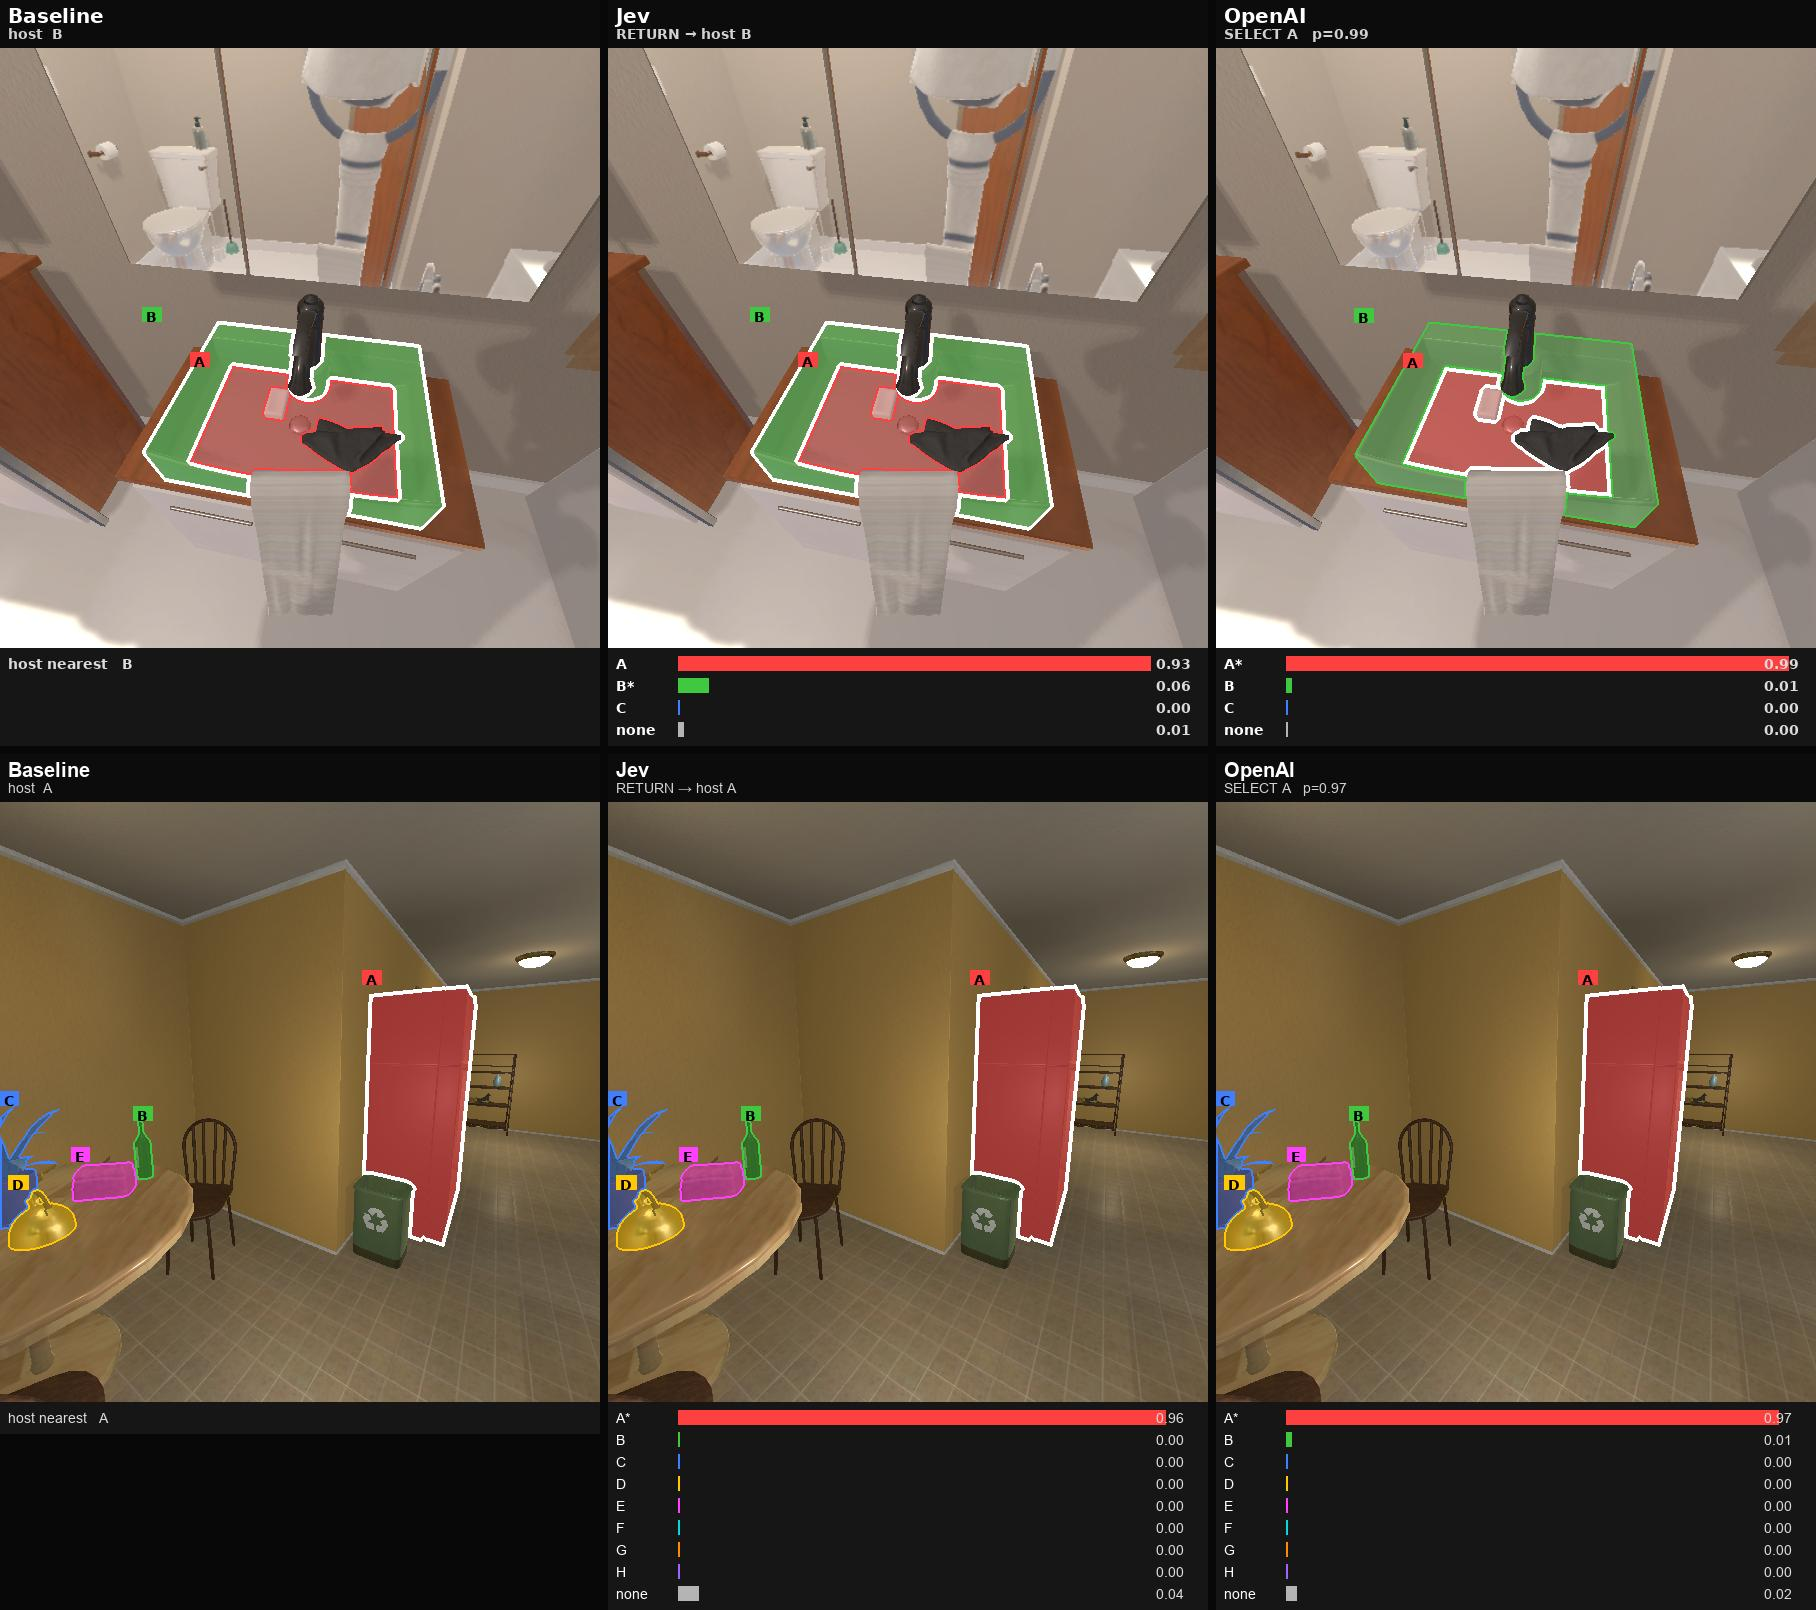
\includegraphics[width=\textwidth]{figs/qual.pdf}
\caption{Two closed-loop Put commits (host / Jev / OpenAI Decisions).
(a)~FloorPlan422, HandTowel into SinkBasin: the host nearest mask is the sink shell (B); Jev RETURNs to it, OpenAI Decisions SELECTs the basin (A).
(b)~FloorPlan7, Put among eight receptacles: OpenAI Decisions SELECTs the fridge (A); Jev RETURNs to the same host mask.} % [CHANGED]
\label{fig:qual}
\end{figure*}

\section{Experiments}
\label{sec:experiments}
\subsection{Setup}
\label{sec:setup}
We insert TRACE on the FILM-adapted and CAPEAM-adapted scorers and run the full ALFRED Oct-21 validation splits ($820$ seen and $821$ unseen episodes, all seven task types) in AI2-THOR~5, following the expert high-level plan and executing each chosen mask by teleporting near the object.
The metadata predicate \texttt{goal\_satisfied()} defines success, so the reported success rate (SR) isolates mask commits under a fixed expert plan; it is \emph{not} the official ALFRED protocol, and published test-set numbers are not comparable.
Four selectors share each host's list: the host, a GT-ID oracle that follows the expert pose when that mask is listed, TRACE\,+\,Jev, and TRACE\,+\,OpenAI Decisions.
A \Diff{} pickup is priced as \texttt{pickup\_not\_ref}; Toggle and Slice execute the host mask. % [CHANGED]
% [KO] TRACE를 FILM 변형과 CAPEAM 변형 점수기에 끼우고 ALFRED Oct-21 전체 검증 분할(seen 820, unseen 821, 일곱 과업 유형 전부)을 AI2-THOR 5에서 돌린다. 전문가 상위 계획을 따르고 선택된 마스크는 객체 근처로 텔레포트해 실행한다. 메타데이터 술어 goal_satisfied()가 성공을 정의하므로 보고하는 SR은 고정된 전문가 계획 아래에서 마스크 확정만 분리한 값이며, 공식 ALFRED 프로토콜이 아니라 공개 테스트셋 수치와 비교할 수 없다. 네 선택기가 각 호스트의 목록을 공유한다: 호스트, 그 마스크가 목록에 있을 때 전문가 포즈를 따르는 GT-ID 오라클, TRACE + Jev, TRACE + OpenAI Decisions. DIFF 집기는 pickup_not_ref로 가격하고 Toggle/Slice는 호스트 마스크를 실행한다.

We report SR, SELECT counts on $N\ge 2$ calls, and commitment regret (CR), the logged extra cost of the executed choice minus that of the oracle decision, with a RETURN charged $B_{\mathrm{ov}}{=}4$; CR measures selection quality, not closed-loop extra cost.
A controlled study fixes $p{=}[0.6,0.4,0]$ and averages a cheap world (wrong-mask extra cost $2$) with an expensive world (extra cost $20$), with detector scores $[0.4,0.9]$ that make the host pick the worse identity, and three synthetic drawings test whether Jev and OpenAI place their mode on the same option.
% [KO] SR, N≥2 호출의 SELECT 수, commitment regret (CR)을 보고한다. CR은 실행된 선택의 기록된 추가 비용에서 오라클 결정의 추가 비용을 뺀 값이고 RETURN에는 B_ov=4를 매기므로 closed-loop 추가 비용이 아니라 선택 품질을 잰다. 통제 연구는 p=[0.6,0.4,0]을 고정하고 싼 세계(추가 비용 2)와 비싼 세계(추가 비용 20)를 평균하며 검출 점수 [0.4,0.9]는 호스트가 더 나쁜 동일성을 고르게 한다. 세 합성 그림은 Jev와 OpenAI가 같은 선택지에 최빈값을 두는지 검사한다.

\subsection{Results}
TRACE raises closed-loop success on every split (Table~\ref{tab:thor}).
TRACE\,+\,OpenAI reaches $0.649$ on FILM seen against the host's $0.500$ ($+122$ episodes) and $0.659$ on CAPEAM seen against $0.528$ ($+107$). % [CHANGED]
On unseen houses Jev is highest, at $0.636$ ($+18$) and $0.649$ ($+17$); OpenAI is $0.633$ ($+16$) and $0.642$ ($+11$). % [CHANGED]
Jev reaches $0.615$ on both seen splits ($+94$ FILM, $+71$ CAPEAM). % [CHANGED]
Almost every recovery turns a host failure into a success; the reverse is small next to the net gains in Table~\ref{tab:thor}. % [CHANGED]
The GT-ID oracle follows the expert pose, including sink rims that THOR cannot receive, so it tracks the host and falls below TRACE.
% [KO] TRACE는 모든 분할에서 closed-loop 성공률을 올린다 (표 II). TRACE + OpenAI는 FILM seen에서 호스트 0.500 대비 0.649(+122), CAPEAM seen에서 0.528 대비 0.659(+107)다. unseen은 Jev가 0.636(+18), 0.649(+17)로 더 높고 OpenAI는 0.633(+16), 0.642(+11)이다. Jev seen은 양쪽 0.615(+94, +71)다. 거의 모든 회복은 호스트 실패를 성공으로 바꾼 것이고, 반대는 표 II 순증에 비해 작다. GT-ID 오라클은 THOR가 받을 수 없는 싱크 rim까지 포함해 전문가 포즈를 따르므로 호스트 근처에 머물고 TRACE 아래다.

The gains concentrate on first-put grounding, where same-class or same-furniture receptacles share the list and a wrong Put ends the episode (Table~\ref{tab:task}).
Look is $1.000$ for every selector and is omitted from Table~\ref{tab:task}; Heat stays hard because a host script performs the retrieval and the list often lacks the named microwave; Pick Two rises on the seen split (FILM $0.048{\to}0.121$, CAPEAM $0.097{\to}0.137$) with \Diff{} pickups priced as \texttt{pickup\_not\_ref}. % [CHANGED]
% [KO] 이득은 같은 클래스나 같은 가구의 용기들이 목록을 공유하고 틀린 Put이 에피소드를 끝내는 첫 Put grounding에 집중된다 (표 III). Look은 모든 선택기에서 1.000이라 표 III에서 뺐고, Heat는 호스트 스크립트가 재회수를 수행하고 목록에 지시된 전자레인지가 없는 경우가 많아 여전히 어려우며, Pick Two는 DIFF 집기를 pickup_not_ref로 가격해 seen에서 FILM 0.048→0.121, CAPEAM 0.097→0.137로 오른다.

\begin{table}[!t]
\centering
\caption{Seen-split SR by ALFRED task type for the host, TRACE\,+\,Jev, and TRACE\,+\,OpenAI. Bold is the best in each host group. Look is $1.000$ for every selector and is omitted.} % [CHANGED]
\label{tab:task}
\scriptsize
\setlength{\tabcolsep}{3.5pt}
\begin{tabular}{lcccccc}
\toprule
& \multicolumn{3}{c}{FILM-adapted (seen)} & \multicolumn{3}{c}{CAPEAM-adapted (seen)} \\
\cmidrule(lr){2-4} \cmidrule(lr){5-7}
Type & Host & Jev & OpenAI & Host & Jev & OpenAI \\
\midrule
pick-and-place & 0.507 & 0.775 & \textbf{0.880} & 0.570 & 0.761 & \textbf{0.880} \\
movable recep.\ & 0.435 & 0.539 & \textbf{0.609} & 0.391 & 0.530 & \textbf{0.609} \\
pick-two       & 0.048 & 0.097 & \textbf{0.121} & 0.097 & 0.097 & \textbf{0.137} \\
clean          & 0.705 & \textbf{0.866} & \textbf{0.866} & 0.839 & \textbf{0.920} & \textbf{0.920} \\
heat           & 0.065 & \textbf{0.140} & 0.121 & 0.047 & \textbf{0.121} & 0.112 \\
cool           & 0.810 & 0.905 & \textbf{0.937} & 0.810 & 0.897 & \textbf{0.944} \\
\bottomrule
\end{tabular}
\end{table}

The gate and a threshold choose different masks on the same belief (Table~\ref{tab:rules}): a low threshold SELECTs in the expensive world, a high threshold RETURNs in the cheap world, and TRACE SELECTs only in the cheap world, where $R(i){<}B_{\mathrm{ov}}$.
The table shows that the rules choose different masks, not that TRACE realizes lower extra cost when RETURN executes the host.
Two closed-loop episodes show the same split (Fig.~\ref{fig:qual}): a bathroom HandTowel Put with a rim and a basin is a cheap world, where OpenAI places $p{\approx}0.99$ on the basin and SELECTs it while the host would have put on the rim; a kitchen Put among eight receptacles with a far fridge is expensive unless $p$ is sharp, so OpenAI's $p{\approx}0.97$ SELECTs the fridge while Jev's flatter belief RETURNs to the same host mask.
% [KO] 게이트와 임계값은 같은 믿음에서 다른 마스크를 고른다 (표 IV). 낮은 임계값은 비싼 세계에서 SELECT하고, 높은 임계값은 싼 세계에서 RETURN하며, TRACE는 R(i)<B_ov인 싼 세계에서만 SELECT한다. 표는 규칙들이 다른 마스크를 고른다는 것을 보일 뿐, RETURN이 호스트를 실행할 때 TRACE의 실현 추가 비용이 더 낮다는 것을 보이지는 않는다. closed-loop 에피소드 두 개가 같은 분기를 보인다 (그림 5). rim과 basin이 있는 욕실 HandTowel Put은 싼 세계로, OpenAI는 basin에 p≈0.99를 두고 SELECT하며 호스트라면 rim에 놓았을 것이다. 먼 냉장고가 있는 여덟 용기 중의 부엌 Put은 p가 뾰족하지 않으면 비싸므로, OpenAI의 p≈0.97은 냉장고를 SELECT하고 Jev의 더 평평한 믿음은 같은 호스트 마스크로 RETURN한다.

\begin{table}[!t]
\centering
\caption{Same belief $p{=}[0.6,0.4,0]$, $B_{\mathrm{ov}}{=}4$. Mean extra cost over a cheap world (wrong-mask extra cost $2$) and an expensive world (extra cost $20$), with RETURN charged $B_{\mathrm{ov}}$ (fixed) or the extra cost of $i_{\mathrm{host}}$ (host). Detector scores $[0.4,0.9]$ make the host pick the worse identity.}
\label{tab:rules}
\scriptsize
\setlength{\tabcolsep}{3.5pt}
\begin{tabular}{lcccc}
\toprule
Rule & Cheap & Expensive & Mean (fixed) & Mean (host) \\
\midrule
TRACE (ours) & SELECT $0$ & RETURN & \textbf{2.4} & 6.4 \\
threshold $\tau{=}0.55$ & SELECT $0$ & SELECT $0$ & 4.4 & \textbf{4.4} \\
threshold $\tau{=}0.75$ & RETURN & RETURN & 4.0 & 6.6 \\
host score & wrong mask & wrong mask & 6.6 & 6.6 \\
\bottomrule
\end{tabular}
\end{table}

The two decision models agree on identity in the three synthetic drawings (accuracy $1.00$, top-1 agreement $1.00$); their beliefs differ most on the absent referent ($L_1{=}0.64$), where Jev assigns $0.88$ to \texttt{none} and OpenAI $0.56$, yet the TRACE decision agrees on every drawing.
Jev has the lower Put CR on three of four splits (Table~\ref{tab:putcr}), consistent with its fewer SELECTs; OpenAI commits more often and has the higher CR on every split, the price of its larger seen SR lift. % [CHANGED]
% [KO] 두 결정 모델은 세 합성 그림에서 동일성에 합의한다 (정확도 1.00, top-1 일치 1.00). 두 믿음은 참조 부재에서 가장 다르며 (L1=0.64) Jev는 none에 0.88, OpenAI는 0.56을 주지만 TRACE 결정은 모든 그림에서 일치한다. Jev는 네 분할 중 셋에서 더 낮은 Put CR을 갖고 (표 V) 이는 더 적은 SELECT와 일치한다. OpenAI는 더 자주 확정하고 모든 분할에서 CR이 더 높으며, 이는 seen SR 상승의 대가다.

\begin{table}[!t]
\centering
\caption{Put commitment regret (CR$\downarrow$) on $N\ge 2$ events over the full Oct-21 splits; RETURN is charged $B_{\mathrm{ov}}{=}4$. Bold is the lowest in each column.}
\label{tab:putcr}
\scriptsize
\setlength{\tabcolsep}{4pt}
\begin{tabular}{lcccc}
\toprule
& \multicolumn{2}{c}{FILM-adapted} & \multicolumn{2}{c}{CAPEAM-adapted} \\
\cmidrule(lr){2-3} \cmidrule(lr){4-5}
Method & seen & unseen & seen & unseen \\
\midrule
Host (baseline) & 2.74 & \textbf{0.44} & 3.41 & 1.92 \\
Always-return & 3.74 & 3.67 & 3.73 & 3.66 \\
TRACE + Jev & \textbf{1.64} & 1.38 & \textbf{1.62} & \textbf{1.47} \\
TRACE + OpenAI & 3.00 & 1.66 & 2.99 & 1.74 \\
\bottomrule
\end{tabular}
\end{table}

\section{Conclusion}
Embodied instruction following turns a class name into one physical instance, or one receptacle part, and guessing wrong does not cost a constant amount.
TRACE prices that commit with a belief over $N{+}1$ hypotheses, an extra-cost matrix $C_r$, and a gate that overrides the host only when a unique mask has expected regret below a local-recovery budget.
On a THOR~5 port of the full Oct-21 validation splits under expert plans, TRACE\,+\,OpenAI raises closed-loop SR from $0.500$ to $0.649$ on FILM seen and from $0.528$ to $0.659$ on CAPEAM seen, mainly on first-put grounding such as basin versus rim. % [CHANGED]
The same belief is cheap in one scene and expensive in another, so a fixed probability threshold cannot make the override decision; the belief-weighted extra cost can.
TRACE still depends on the host list, on action-success memory, and on the quality of $p$ and $C_r$; tighter critics and stronger detectors would improve what the gate consumes.
% [KO] 체화된 지시 수행은 클래스 이름을 하나의 물리적 인스턴스나 용기 부위로 바꾸며, 잘못 추측하는 비용은 일정하지 않다. TRACE는 그 확정을 N+1개 가설에 대한 믿음, 추가 비용 행렬 C_r, 유일한 마스크의 기대 후회가 가까운 복구 예산보다 작을 때만 호스트를 덮어쓰는 게이트로 가격한다. 전문가 계획 아래 Oct-21 전체 검증 분할의 THOR 5 이식에서 TRACE + OpenAI는 closed-loop SR을 FILM seen 0.500→0.649, CAPEAM seen 0.528→0.659로 올렸고 주로 basin 대 rim 같은 첫 Put grounding에서다. 같은 믿음이 한 장면에서는 싸고 다른 장면에서는 비싸므로 고정 확률 임계값은 덮어쓰기 결정을 내릴 수 없고, 믿음으로 가중한 추가 비용은 내릴 수 있다. TRACE는 여전히 호스트 목록, 행동 성공 메모리, p와 C_r의 품질에 의존하며, 더 촘촘한 평가기와 더 강한 검출기는 게이트가 소비하는 것을 개선할 것이다.

\bibliographystyle{IEEEtran}
\bibliography{references}
\end{document}
